\section{Notaciones del dia de hoy}
    
\begin{figure}[H]
\centering
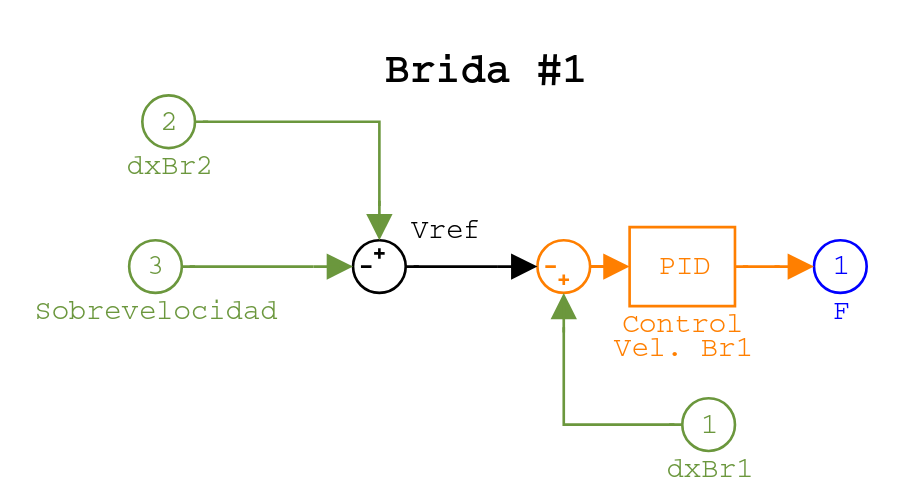
\includegraphics[width=1\linewidth]{include/brida_simulink.png}
\caption{Diagra de simulink de la brida 1 sacado de la facultad de Quilmes}
\label{}
\end{figure}

Para la anterior figura, concluimos la siguiente ecuacion dinamica

\begin{equation}
\begin{cases} 
M \cdot \dot{v_1} + f_r \cdot v_1 = T_{ce} - T_{def} - \left[ k \cdot (v_1 + s_v - v_2) + k_I * \theta + k_D \cdot(v_1 + s_v - v_2)' \right]\\
\dot{\theta} = v_1 + s_v - v_2

\end{cases}
\end{equation}

donde $v_1$ es la velocidad de brida 1, $s_v$ es la sobrevelocidad, $v_2$ es la 
velocidad de la brida 2.

\begin{figure}[H]
\centering
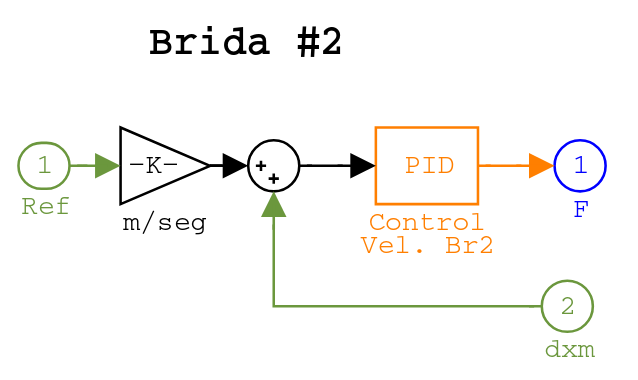
\includegraphics[width=1\linewidth]{include/brida_2_simulink.png}
\caption{Diagra de simulink de la brida 2 sacado de la facultad de Quilmes}
\label{}
\end{figure}

Para la anterior figura, concluimos la siguiente ecuacion dinamica

\begin{equation}
\begin{cases} 

    m_2 \cdot \dot{v_{2}} + f_{r2} \cdot v_{2} = T_{H} - T_{ce} + F_2(v_3 - v_{2}) \\
    \dot{\theta ^2} = v_3 - v_{2}

\end{cases}
\end{equation}

donde 

\begin{equation}
    F_2(v_3 - v_{2}) = - \left[ k^2 (v_3 - v_{2}) + k^2_I \cdot \theta ^2 + k^2_d \cdot( v_3 - v_{2})' \right]
\end{equation}

el supra $2$ solo indica que es otra varibale, no una potencia.

Algo para recordar, en el texto dice $V_{ref}$ pero para nosotros es $V_3$
